\KOMAoptions{twoside=semi}
\begin{titlepage}
    {\Huge\raggedright Introduction to Linear Algebra \par}
    {\Large\raggedright \textit{with Earth Science Applications} \hfill\textcolor{Mahogany}{\rule{3mm}{3mm}} \par}
    \vspace{3mm}\hrule\par
    {\Large\raggedleft First Edition \hfill C.L. Loi \par}
    \vfill
    {\Large\raggedleft A student from\\
    CUHK-EESC/NTU-AS \par}
\end{titlepage}

\begin{titlepage}
\begin{center}
Introduction to Linear Algebra with Earth Science Applications

Copyright ©, C.L. Loi, 2025

All rights reserved. Any reproduction of this work, in part or in whole, is prohibited without the written permission of the author.
\end{center}
\vfill
First Edition, e-book, Self-published (May 2025)
%First Edition, Hardcover, Self-published (May 2025) \\
%ISBN: 978-626-01-3990-2
\end{titlepage}

\KOMAoptions{twoside=semi}

\chapter*{Preface}
This is a Linear Algebra textbook specifically designed for students who are majoring in any Earth Science-related subjects like Geophysics and Atmospheric Sciences, and are also interested in Mathematics. With these target readers in mind, we set out to provide an adequate treatment of Linear Algebra concepts that enables them to tackle relevant Earth Science problems. In each chapter, we focus on a selected Linear Algebra topic, motivated by Earth Science examples and supplemented with Python programming tutorials. At the end of each chapter, a number of exercises are given for elucidating the concepts and working on Earth Science projects. \par
{\raggedleft C.L. Loi \par}
\textit{Acknowledgement: This work is also partially supported by the grants from NSTC (112-2123-M-002-002, 113-2639-M-002-008-ASP) as the author is working at TDRC, NTU-AS.}\par
The tex/pdf files and Python scripts can be found on the GitHub repository:\\ \href{https://github.com/BenjaminGor/Intro_to_LinAlg_Earth}{https://github.com/BenjaminGor/Intro\_to\_LinAlg\_Earth}.

\chapter*{Forewords}

It is my pleasure to recommend this special textbook to you. I appreciate this book from both a personal level and from a professional perspective.

C. L. Loi, the author of this book, was my Master's degree graduate student and is currently a member of the research staff in my research group, Typhoon Dynamics Research Center. In addition to his excellent research work on using machine learning to enhance the understanding of tropical cyclogenesis and to investigate the predictability of tropical cyclone density in the subseasonal-to-seasonal reforecast, C. L. dedicated tremendous time and efforts in the preparation and writing of this textbook over the past two years. I am truly impressed with his perseverance and the quality of his work.

Linear Algebra plays a crucial role in the study of Earth Science as a mathematical tool to analyze and model natural and simulated phenomena, from geophysical and geomechanics studies, remote sensing to climate modeling and beyond. I believe that readers, especially students interested in Earth Science problems, would find this textbook a clear and in-depth guide that is highly applicable to their studies. Below are some of the values that I find in this book and trust would benefit you as a reader.

\begin{itemize}
    \item A very solid and comprehensive review of Linear Algebra,
    \item Close examination of the core concepts and detailed proofs,
    \item Connections to Earth Science applications, such as 
    \begin{itemize}
        \item Empirical Orthogonal Functions to decompose El Niño-Southern Oscillation (ENSO) modes;
        \item Special polynomial solutions for equatorial waves;
        \item Fourier analysis of Sea Surface Temperature (SST) time series;
        \item Singular Value Decomposition (SVD) for data compression;
        \item Investigation of dynamical systems like the Lorenz-63 model; as well as
        \item Continuum Mechanics and Data Assimilation.
    \end{itemize}
\end{itemize}

Overall, this is a high-quality, uncommon effort from a very hard-working researcher, intended for Earth Science students but can also benefit those who are looking to learn the fundamental concepts and applications of Linear Algebra. I highly recommend this book and hope you enjoy the reading and grow in your learning!

{\raggedleft Chun-Chieh Wu\\
Chair Professor, Department of Atmospheric Sciences,\\
National Taiwan University \par}

\newpage

This book, compiled by our alumni Benjamin Loi, delves into the application of Linear Algebra in the field of Earth Sciences and provides a solid mathematical foundation along with practical insights. As one of the core areas of mathematics, Linear Algebra plays a crucial role in various scientific disciplines, particularly in Earth and Atmospheric Sciences. The purpose of this book is to help readers establish a strong foundation in Linear Algebra and guide them on how to effectively apply these mathematical concepts to real-world problems in Earth Sciences.

In addition to a thorough exploration of the mathematical theories, the author also includes many Python programming tutorials, which are immensely helpful for both academic research and practical applications. Whether you are a course instructor or an undergraduate student, this book offers valuable resources to help enhance your skills in both academic and practical settings.

The content of this book can also serve as a textbook or tutorial material for course design or teaching support. It is not only valuable to scholars in Earth Sciences but also to students interested in mathematics and programming, offering a challenging and inspiring learning resource.

We hope that readers will find inspiration in this book and apply the theories and methods of Linear Algebra to real-world problems. We believe this will help them achieve greater success in their academic or professional careers.

{\raggedleft Man Nin Chan\\
Associate Professor, Department of Earth and Environmental Sciences,\\
The Chinese University of Hong Kong \par}

\chapter*{Preface (the Heartfelt Version)}
I have toiled for almost one-and-a-half years to deliver this work. This project started from a small Linear Algebra workshop I gave at CUHK-EESC (previously ESSC) in 2021. The initial draft was only 200 pages long and very immature (same as me back then, lol!). After finishing my Master's degree in 2023 at NTU-AS, I decided to resume the writing of this book. Little did I know at that moment I had taken on a very long and epic journey. In the early beginning, I advanced very quickly, but soon got stuck in the "Saggy Middle". It was absolutely no easy task to produce a Mathematical textbook with 18 chapters, and merely looking at this goal could be disheartening and overwhelming. Sometimes, I struggled to produce even only one page a day. More often than not, I considered the option of giving up, wondering if I really could see the finishing of this work. However, thanks to my stubbornness, I was too proud to kneel: I had a burning desire to finish what I started and show it to the world. Perhaps deep in my heart, I really wanted to get praised for my effort and intelligence, to prove to others that I was a force to be reckoned with. Don't get me wrong, I am still aiming for these rewards. However, along my writer's journey, I have also earned and learned far more precious things and important lessons.

I have become much more resilient and persevering. I disciplined myself to write (almost) every day despite all the ups and downs happening in my life. Many less-than-happy and discouraging events occurred to me, e.g.\ relationships and personal well-being, but I have weathered the storm and come back stronger every time.

I have also become more grateful for the supportive people around me. Without their help, this book (as well as me) would never have survived and got to this stage. I guess one of the reasons why I persisted in completing this book was that I did not want to let them down and must return their favors.

Finally, I have realized my true potential and determination. I am much more capable than I ever imagined. For a long time, I was pathetic, but now I have found my passion and dream. I confronted my fear whenever I wrote. I am no longer a little shepherd: I am now a mighty, wise ruler who has managed to overcome Goliath! (As an afterthought, all of these are fully due to God's grace.)

I wholeheartedly hope that as you read this book, apart from learning the knowledge of Linear Algebra, you will feel my soul and excitement, appreciate the enormous efforts that were put into it, and have a glimpse of my growth and transformation. So, let me conclude this with a quote.

\begin{center}
\large
"Every secret of a writer's soul, every experience of his life, every quality of his mind is written large in his works."\\
-- Virginia Woolf
\end{center}

{\raggedleft Sincerely,\\
Benjamin \par}

\chapter*{Dedications}

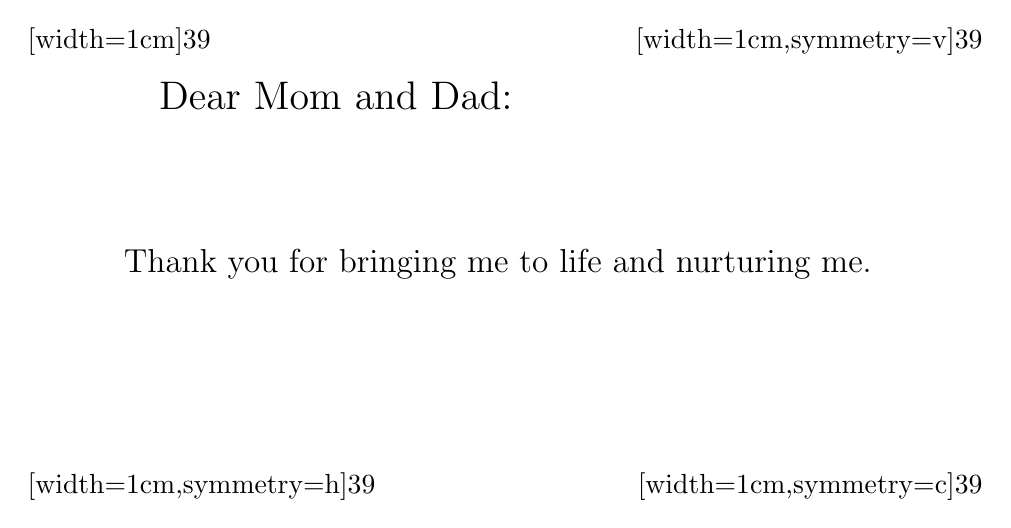
\begin{tikzpicture}[every node/.style={inner sep=0pt}]
\node[minimum width = \textwidth, minimum height = 6cm, align = left](vecbox){\large
Thank you for bringing me to life and nurturing me.
};
\node[anchor=north west](CNW) at (vecbox.north west)
{\pgfornament[width=1cm]{39}};
\node[anchor=north west, xshift=0.5cm, yshift=-0.5cm] at (CNW) {\Large Dear Mom and Dad:};
\node[anchor=north east](CNE) at (vecbox.north east)
{\pgfornament[width=1cm,symmetry=v]{39}};
\node[anchor=south west](CSW) at (vecbox.south west)
{\pgfornament[width=1cm,symmetry=h]{39}};
\node[anchor=south east](CSE) at (vecbox.south east)
{\pgfornament[width=1cm,symmetry=c]{39}};
\pgfornamenthline{CNW}{CNE}{north}{88}
\pgfornamenthline{CSW}{CSE}{south}{88}
\pgfornamentvline{CNW}{CSW}{west}{88}
\pgfornamentvline{CNE}{CSE}{east}{88}
\end{tikzpicture}

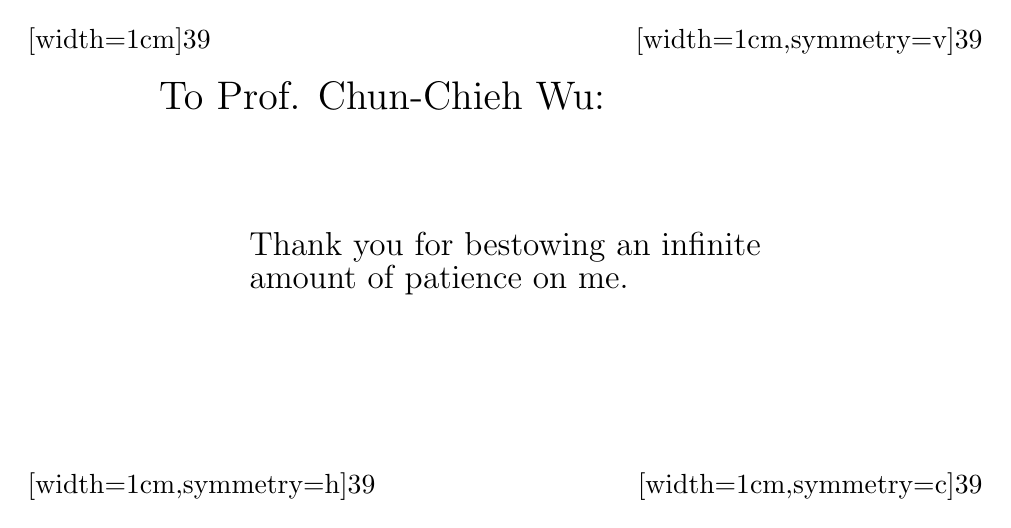
\begin{tikzpicture}[every node/.style={inner sep=0pt}]
\node[minimum width = \textwidth, minimum height = 6cm, align = left,](vecbox){\large
Thank you for bestowing an infinite \\ \large amount of patience on me.
};
\node[anchor=north west](CNW) at (vecbox.north west)
{\pgfornament[width=1cm]{39}};
\node[anchor=north west, xshift=0.5cm, yshift=-0.5cm] at (CNW) {\Large To Prof. Chun-Chieh Wu:};
\node[anchor=north east](CNE) at (vecbox.north east)
{\pgfornament[width=1cm,symmetry=v]{39}};
\node[anchor=south west](CSW) at (vecbox.south west)
{\pgfornament[width=1cm,symmetry=h]{39}};
\node[anchor=south east](CSE) at (vecbox.south east)
{\pgfornament[width=1cm,symmetry=c]{39}};
\pgfornamenthline{CNW}{CNE}{north}{88}
\pgfornamenthline{CSW}{CSE}{south}{88}
\pgfornamentvline{CNW}{CSW}{west}{88}
\pgfornamentvline{CNE}{CSE}{east}{88}
\end{tikzpicture}

\newpage

\vspace*{10pt}

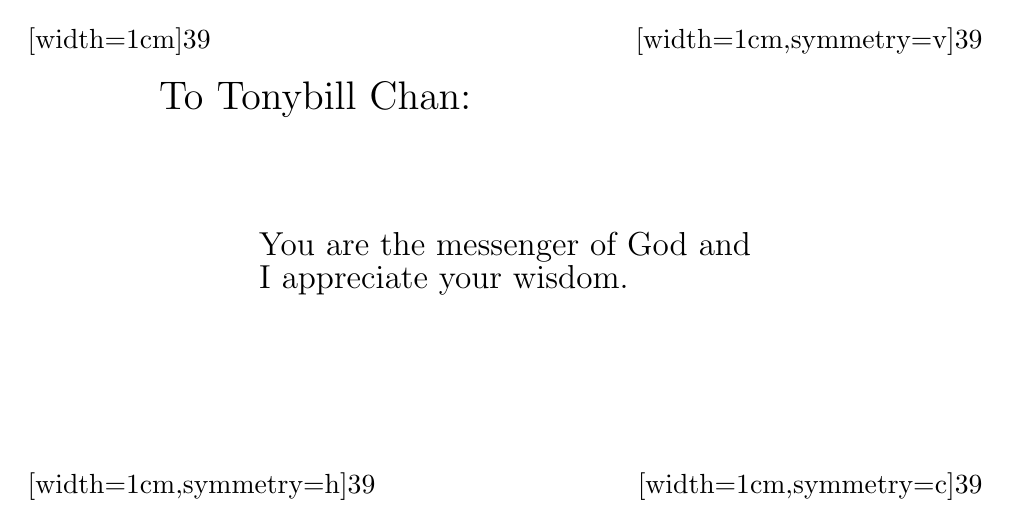
\begin{tikzpicture}[every node/.style={inner sep=0pt}]
\node[minimum width = \textwidth, minimum height = 6cm, align = left](vecbox){\large
You are the messenger of God and \\ \large I appreciate your wisdom.
};
\node[anchor=north west](CNW) at (vecbox.north west)
{\pgfornament[width=1cm]{39}};
\node[anchor=north west, xshift=0.5cm, yshift=-0.5cm] at (CNW) {\Large To Tonybill Chan:};
\node[anchor=north east](CNE) at (vecbox.north east)
{\pgfornament[width=1cm,symmetry=v]{39}};
\node[anchor=south west](CSW) at (vecbox.south west)
{\pgfornament[width=1cm,symmetry=h]{39}};
\node[anchor=south east](CSE) at (vecbox.south east)
{\pgfornament[width=1cm,symmetry=c]{39}};
\pgfornamenthline{CNW}{CNE}{north}{88}
\pgfornamenthline{CSW}{CSE}{south}{88}
\pgfornamentvline{CNW}{CSW}{west}{88}
\pgfornamentvline{CNE}{CSE}{east}{88}
\end{tikzpicture}

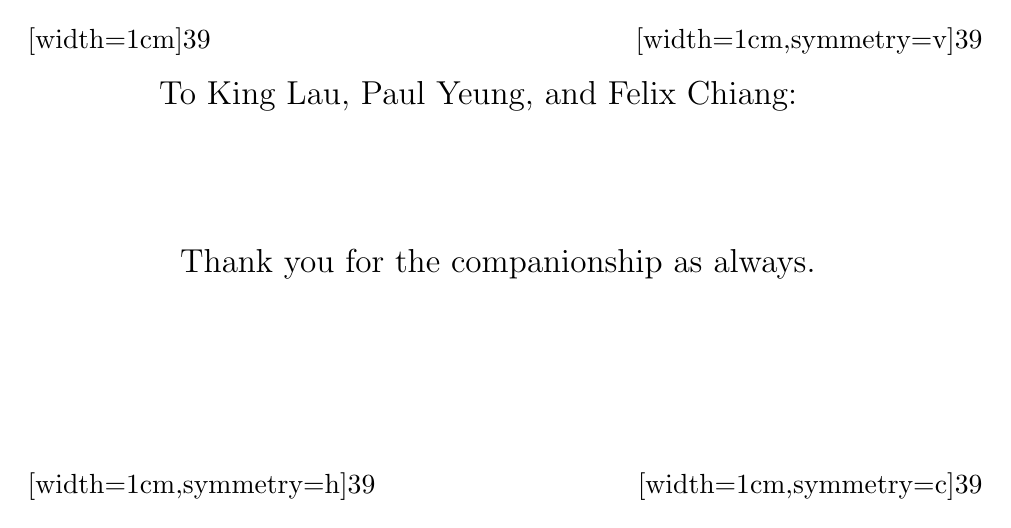
\begin{tikzpicture}[every node/.style={inner sep=0pt}]
\node[minimum width = \textwidth, minimum height = 6cm, align = left](vecbox){\large
Thank you for the companionship as always.
};
\node[anchor=north west](CNW) at (vecbox.north west)
{\pgfornament[width=1cm]{39}};
\node[anchor=north west, xshift=0.5cm, yshift=-0.5cm] at (CNW) {\large To King Lau, Paul Yeung, and Felix Chiang:};
\node[anchor=north east](CNE) at (vecbox.north east)
{\pgfornament[width=1cm,symmetry=v]{39}};
\node[anchor=south west](CSW) at (vecbox.south west)
{\pgfornament[width=1cm,symmetry=h]{39}};
\node[anchor=south east](CSE) at (vecbox.south east)
{\pgfornament[width=1cm,symmetry=c]{39}};
\pgfornamenthline{CNW}{CNE}{north}{88}
\pgfornamenthline{CSW}{CSE}{south}{88}
\pgfornamentvline{CNW}{CSW}{west}{88}
\pgfornamentvline{CNE}{CSE}{east}{88}
\end{tikzpicture}

\vspace*{\fill}

\newpage

\vspace*{10pt}

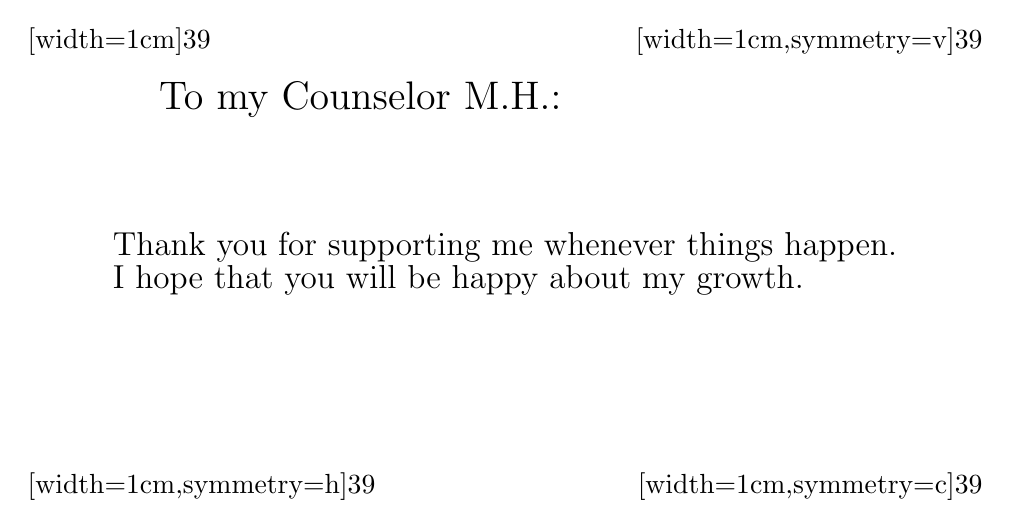
\begin{tikzpicture}[every node/.style={inner sep=0pt}]
\node[minimum width = \textwidth, minimum height = 6cm, align = left](vecbox){\large
Thank you for supporting me whenever things happen. \\
\large I hope that you will be happy about my growth.
};
\node[anchor=north west](CNW) at (vecbox.north west)
{\pgfornament[width=1cm]{39}};
\node[anchor=north west, xshift=0.5cm, yshift=-0.5cm] at (CNW) {\Large To my Counselor M.H.:};
\node[anchor=north east](CNE) at (vecbox.north east)
{\pgfornament[width=1cm,symmetry=v]{39}};
\node[anchor=south west](CSW) at (vecbox.south west)
{\pgfornament[width=1cm,symmetry=h]{39}};
\node[anchor=south east](CSE) at (vecbox.south east)
{\pgfornament[width=1cm,symmetry=c]{39}};
\pgfornamenthline{CNW}{CNE}{north}{88}
\pgfornamenthline{CSW}{CSE}{south}{88}
\pgfornamentvline{CNW}{CSW}{west}{88}
\pgfornamentvline{CNE}{CSE}{east}{88}
\end{tikzpicture}

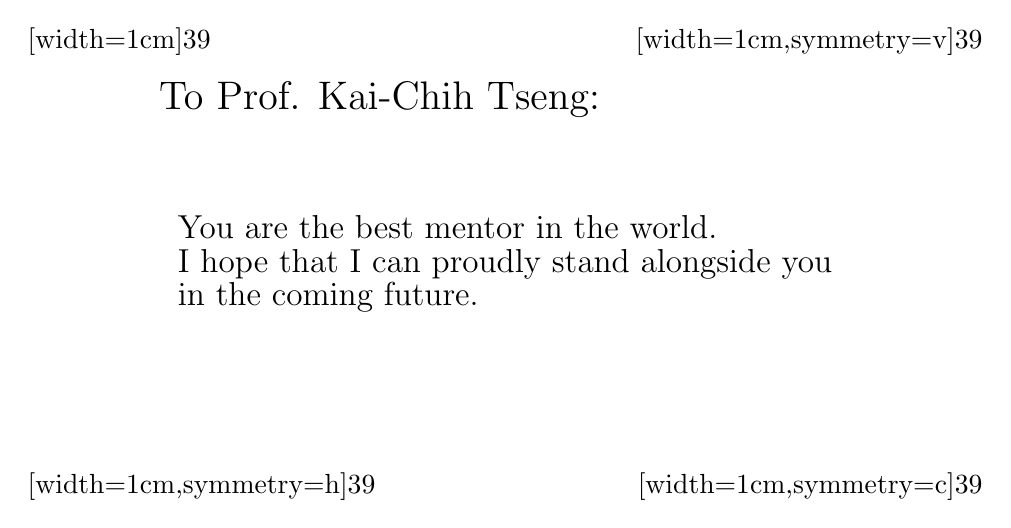
\begin{tikzpicture}[every node/.style={inner sep=0pt}]
\node[minimum width = \textwidth, minimum height = 6cm, align = left](vecbox){\large
You are the best mentor in the world. \\
\large I hope that I can proudly stand alongside you \\ \large in the coming future.
};
\node[anchor=north west](CNW) at (vecbox.north west)
{\pgfornament[width=1cm]{39}};
\node[anchor=north west, xshift=0.5cm, yshift=-0.5cm] at (CNW) {\Large To Prof. Kai-Chih Tseng:};
\node[anchor=north east](CNE) at (vecbox.north east)
{\pgfornament[width=1cm,symmetry=v]{39}};
\node[anchor=south west](CSW) at (vecbox.south west)
{\pgfornament[width=1cm,symmetry=h]{39}};
\node[anchor=south east](CSE) at (vecbox.south east)
{\pgfornament[width=1cm,symmetry=c]{39}};
\pgfornamenthline{CNW}{CNE}{north}{88}
\pgfornamenthline{CSW}{CSE}{south}{88}
\pgfornamentvline{CNW}{CSW}{west}{88}
\pgfornamentvline{CNE}{CSE}{east}{88}
\end{tikzpicture}

\vspace*{\fill}

%\setcounter{tocdepth}{1}
\tableofcontents